\documentclass[10pt]{article}
\usepackage[utf8]{inputenc}
\usepackage{listings}
\usepackage{xcolor}
\usepackage{subcaption}
\usepackage{longtable}
\usepackage{booktabs}
\usepackage{enumitem}
\usepackage{hyperref}
\hypersetup{
	colorlinks,
	citecolor=black,
	filecolor=black,
	linkcolor=black,
	urlcolor=black
}

\definecolor{codegreen}{rgb}{0,0.6,0}
\definecolor{codegray}{rgb}{0.5,0.5,0.5}
\definecolor{codepurple}{rgb}{0.58,0,0.82}
\definecolor{backcolour}{rgb}{0.95,0.95,0.92}
\usepackage{color}   %May be necessary if you want to color links
\usepackage{hyperref}
\usepackage{graphicx}
\graphicspath{ {./images/} }
\hypersetup{
    colorlinks=true, %set true if you want colored links
    linktoc=all,     %set to all if you want both sections and subsections linked
    linkcolor=black,  %choose some color if you want links to stand out
    urlcolor=blue,
}
\lstdefinestyle{mystyle}{
    backgroundcolor=\color{backcolour},   
    commentstyle=\color{codegreen},
    keywordstyle=\color{magenta},
    numberstyle=\tiny\color{codegray},
    stringstyle=\color{codepurple},
    basicstyle=\ttfamily\footnotesize,
    breakatwhitespace=false,         
    breaklines=true,                 
    captionpos=b,                    
    keepspaces=true,                 
    numbers=left,                    
    numbersep=5pt,                  
    showspaces=false,                
    showstringspaces=false,
    showtabs=false,                  
    tabsize=2
}

\lstset{style=mystyle}

\title{RASD}
\author{Mauro Famà, Giacomo Lombardo}
%\date{October 2021}

\begin{document}
\thispagestyle{empty}
\begin{titlepage}
    \begin{center}
       %\vspace*{2cm}
       {\Huge \textbf{RASD}} %%Replace this with the Title of your research
       \vspace{0.5cm}
       \\
    \begin{LARGE}
        {Requirements Analysis and Specification Document}
        \vspace{1.0cm}
        \\
        
\includegraphics[width=13cm]{polimi.png}
        \vspace{1.5cm}\\
        Mauro Famà (10631287)\\Giacomo Lombardo (10674987)
        \vspace{1.5cm}\\
        {A.Y. 2021/2022}
    \end{LARGE}  
   \end{center}
\end{titlepage}
\newpage
\tableofcontents %this command creates an index
\newpage
\section{Introduction}
As world's population is increasing at steady pace, new challenges arise with its growth.
Accordingly to a recent UN estimate, by 2050 globally there will be almost 10 billion people, 
and food demand is expected to increase between 59\% to 98\%. Furthermore, climate change is causing 
problems to the agriculture that are getting bigger every year: its effect is predicted to result in a 
4\%-26\% loss by the end of the century in the Indian agricuture sector.\\
To tackle the situation, Telangana's state, which is the 11th biggest state in India, has decided to develop a 
platform to implement anticipatory, data-driven models to strengthen the policies in farming, with the ultimate
goal of increasing the output of the agriculture sector.\\
This is the idea behind DREAM (Data-dRiven prEdictive fArMing), a platform where Telangana's
Policy Makers, farmers and agronomists cooperate in order to enhance agriculture performances and facilitate the 
management of help requests, visits to farms and general communications betweens the actors in this scenario.
\subsection{Purpose}
The purpose of this document is to present a detailed description of the DREAM
 (Data-dRiven PrEdictive FArMing) platform. It will explain the purpose and features of 
 the software, the interfaces of the software, what the software will do and the constraints
  under which it must operate. This document is intended for software users and also 
  potential developers. The description will be offered by using models, providing scenarios and 
  their relative use cases, analyzing most important functional and non-functional requirements.
\subsection{Scope} %qui inserirei overview of the function of the system and the reasons for its development, goals and success criteria
The DREAM platform is intended for use by Telengana's policy makers, farmers and agronomists.\\
DREAM allows Telangana's policy makers, through the use of data provided by farmers regarding goods 
production, to extrapolate significative information and obtain a general view of the food production of the entire region. 
In this way, they will be given a platform to model and monitor the region's food system, facilitating the study and the 
realization of an adequate and well-performing long-term production strategy. The platform will provide policy makers the possibility 
to easily monitor farmers' performance and manage agronomists' interventions whenever and wherever needed. 
Furthermore, they will be able to identify those farmers whose production has been particularly good or bad,
in order to reward the best performing farmers with incentives and to provide help to the farmers in need.\\ 
DREAM's goal is also to provide useful resources and tools to local farmers, who will be given a platform to facilitate 
the farmer-to-farmer and farmer-to-policy maker communication. Via DREAM, farmers will be able to participate to forum
discussions, easily create help requests and obtain sensitive information such as accurate weather forecasts and personalized 
suggestions regarding goods and agriculture routines.\\
For what concerns the local agronomists, DREAM facilitates the daily visit controls scheduling and regulates it accordingly
to farmer needs, increasing the visits whether a farmer performance is significantly lower than the average.\\
In this document, the agronomist perspective won't be analyzed in detail, but it will be considered only marginally and in those
cases where there is a significant interaction between agronomists and the other actors.
\subsubsection{Goals}
\begin{enumerate}[label=\textbf{G\arabic*}]
    \item \label{goal:g1} Allow Telangana's Policy Makers to monitor local agriculture
    \item \label{goal:g2} Allow farmers to receive assistance or rewards based on their performance
    \item \label{goal:g3} Allow farmers to request and receive help
    \item \label{goal:g4} Create a farmer's network to promote collaboration and mutual aid 
    \item \label{goal:g5} Improve farmers' performance and productivit
\end{enumerate}
\subsubsection{World and Machine Phenomena}
\begin{center}
    \vspace{0.5cm}
    \begin{tabular}{|c c|} 
    \hline
    World Phenomena & Description \\ 
    \hline\hline
    WP1 & Crop damage due to natural causes \\ 
    \hline
    WP2 & Heavy meteorological conditions\\ 
    \hline
    WP3 & Agriculture operations and routines\\ 
    \hline
    WP4 & Agricuture product collection \\ 
    \hline
    WP5 & Control visits to farmers \\ 
    \hline
    \end{tabular}
    \vspace{0.5cm}\\
    \begin{tabular}{|c c c|} 
        \hline
        Shared Phenomena & Description & Controlled By\\ 
        \hline\hline
        SP1 & Insertion of crop collection data & W \\ 
        \hline
        SP2 & Visualization of weather forecasts & M \\ 
        \hline
        SP3 & Visualization of suggestions & M \\ 
        \hline
        SP4 & Sending of notifications by TPMs & W \\ 
        \hline
        SP5 & Receiving of notifications by farmers & M \\ 
        \hline
        SP6 & Sending help requests & W \\ 
        \hline
        SP7 & Contribution to a forum discussion & W \\ 
        \hline
        SP8 & Visualization of crop collection data & M \\ 
        \hline
        SP9 & Interview request & W \\ 
        \hline
        SP10 & Agronomist visit request & W \\ 
        \hline
        SP11 & Login/registration on the platform & W \\ 
        \hline
        \end{tabular}
\end{center}
\subsection{Definitions, Acronyms, Abbreviations}
% PM = Policy Maker
\subsection{Revision history}
\subsection{Reference Documents}
\subsection{Document Structure}
\newpage
\section{Overall Description}
\subsection{Product Perspective}
The system will be implemented from scratch, completely replacing the legacy system.
The system will make use of some already existing functionalities, such as in weather forecasting where there is 
already an existing platform for collecting and visualizing data (https://www.tsdps.telangana.gov.in/aws.jsp).
\subsubsection{Class diagram}
The class diagram in \ref{fig:classDiagram} is a high-level representation of the system. The main elements in the diagram are:
\begin{itemize}
    \item \textbf{User}: a user of the DREAM platform. More specifically, a user can be:
    \begin{itemize}
        \item \textbf{Farmer}
        \item \textbf{Policy Maker}
    \end{itemize} 
    \item \textbf{Help Request}: represents a help request created by a farmer and taken in charge by a policy maker.
    \item \textbf{Forum}: represents the platform's forum, containing discussions grouped in threads.
    \item \textbf{Thread}: represents a thread of the forum.
    \item \textbf{Intervention}: represents an intervention in a forum discussion.
    \item \textbf{Terrain}: represents an area of property of a farmer destinated to agricultural use.
    \item \textbf{Sensor}: represents a generic sensor installed in a terrain to retrieve data such as irrigation or soil humidity.
    \item \textbf{Sensor Data}: high level astraction of the data retrieved by sensors and inserted in reports.
    \item \textbf{Product}: represents a generic agricultural product. Products can be subdivided in:
    \begin{itemize}
        \item \textbf{Agricultural Products}: goods produced by farmers (e.g. vegetables).
        \item \textbf{Support Products}: auxiliary products used in goods production (e.g. fertilizers).
    \end{itemize} 
    \item \textbf{Suggestion}: represents a suggestion related to a product.
    \item \textbf{Geographical Area}: represents a wide area containing multiple farmer's terrains. The Telangana territory is subdivided into areas to facilitate the workload division between policy makers.
    \item \textbf{Weather Forecasts}: represents a weather forecast for a specific date. Contains various informations such as weather conditions, sunrise and sunset times, precipitations, etc..
    \item \textbf{Report}: represents a report containing information about goods production, compiled by farmers at the end of the crop collecting phase.
    \item \textbf{Trimester}: represents a trimester of a year.
\end{itemize}
\begin{figure}[ht!]
    \centering
    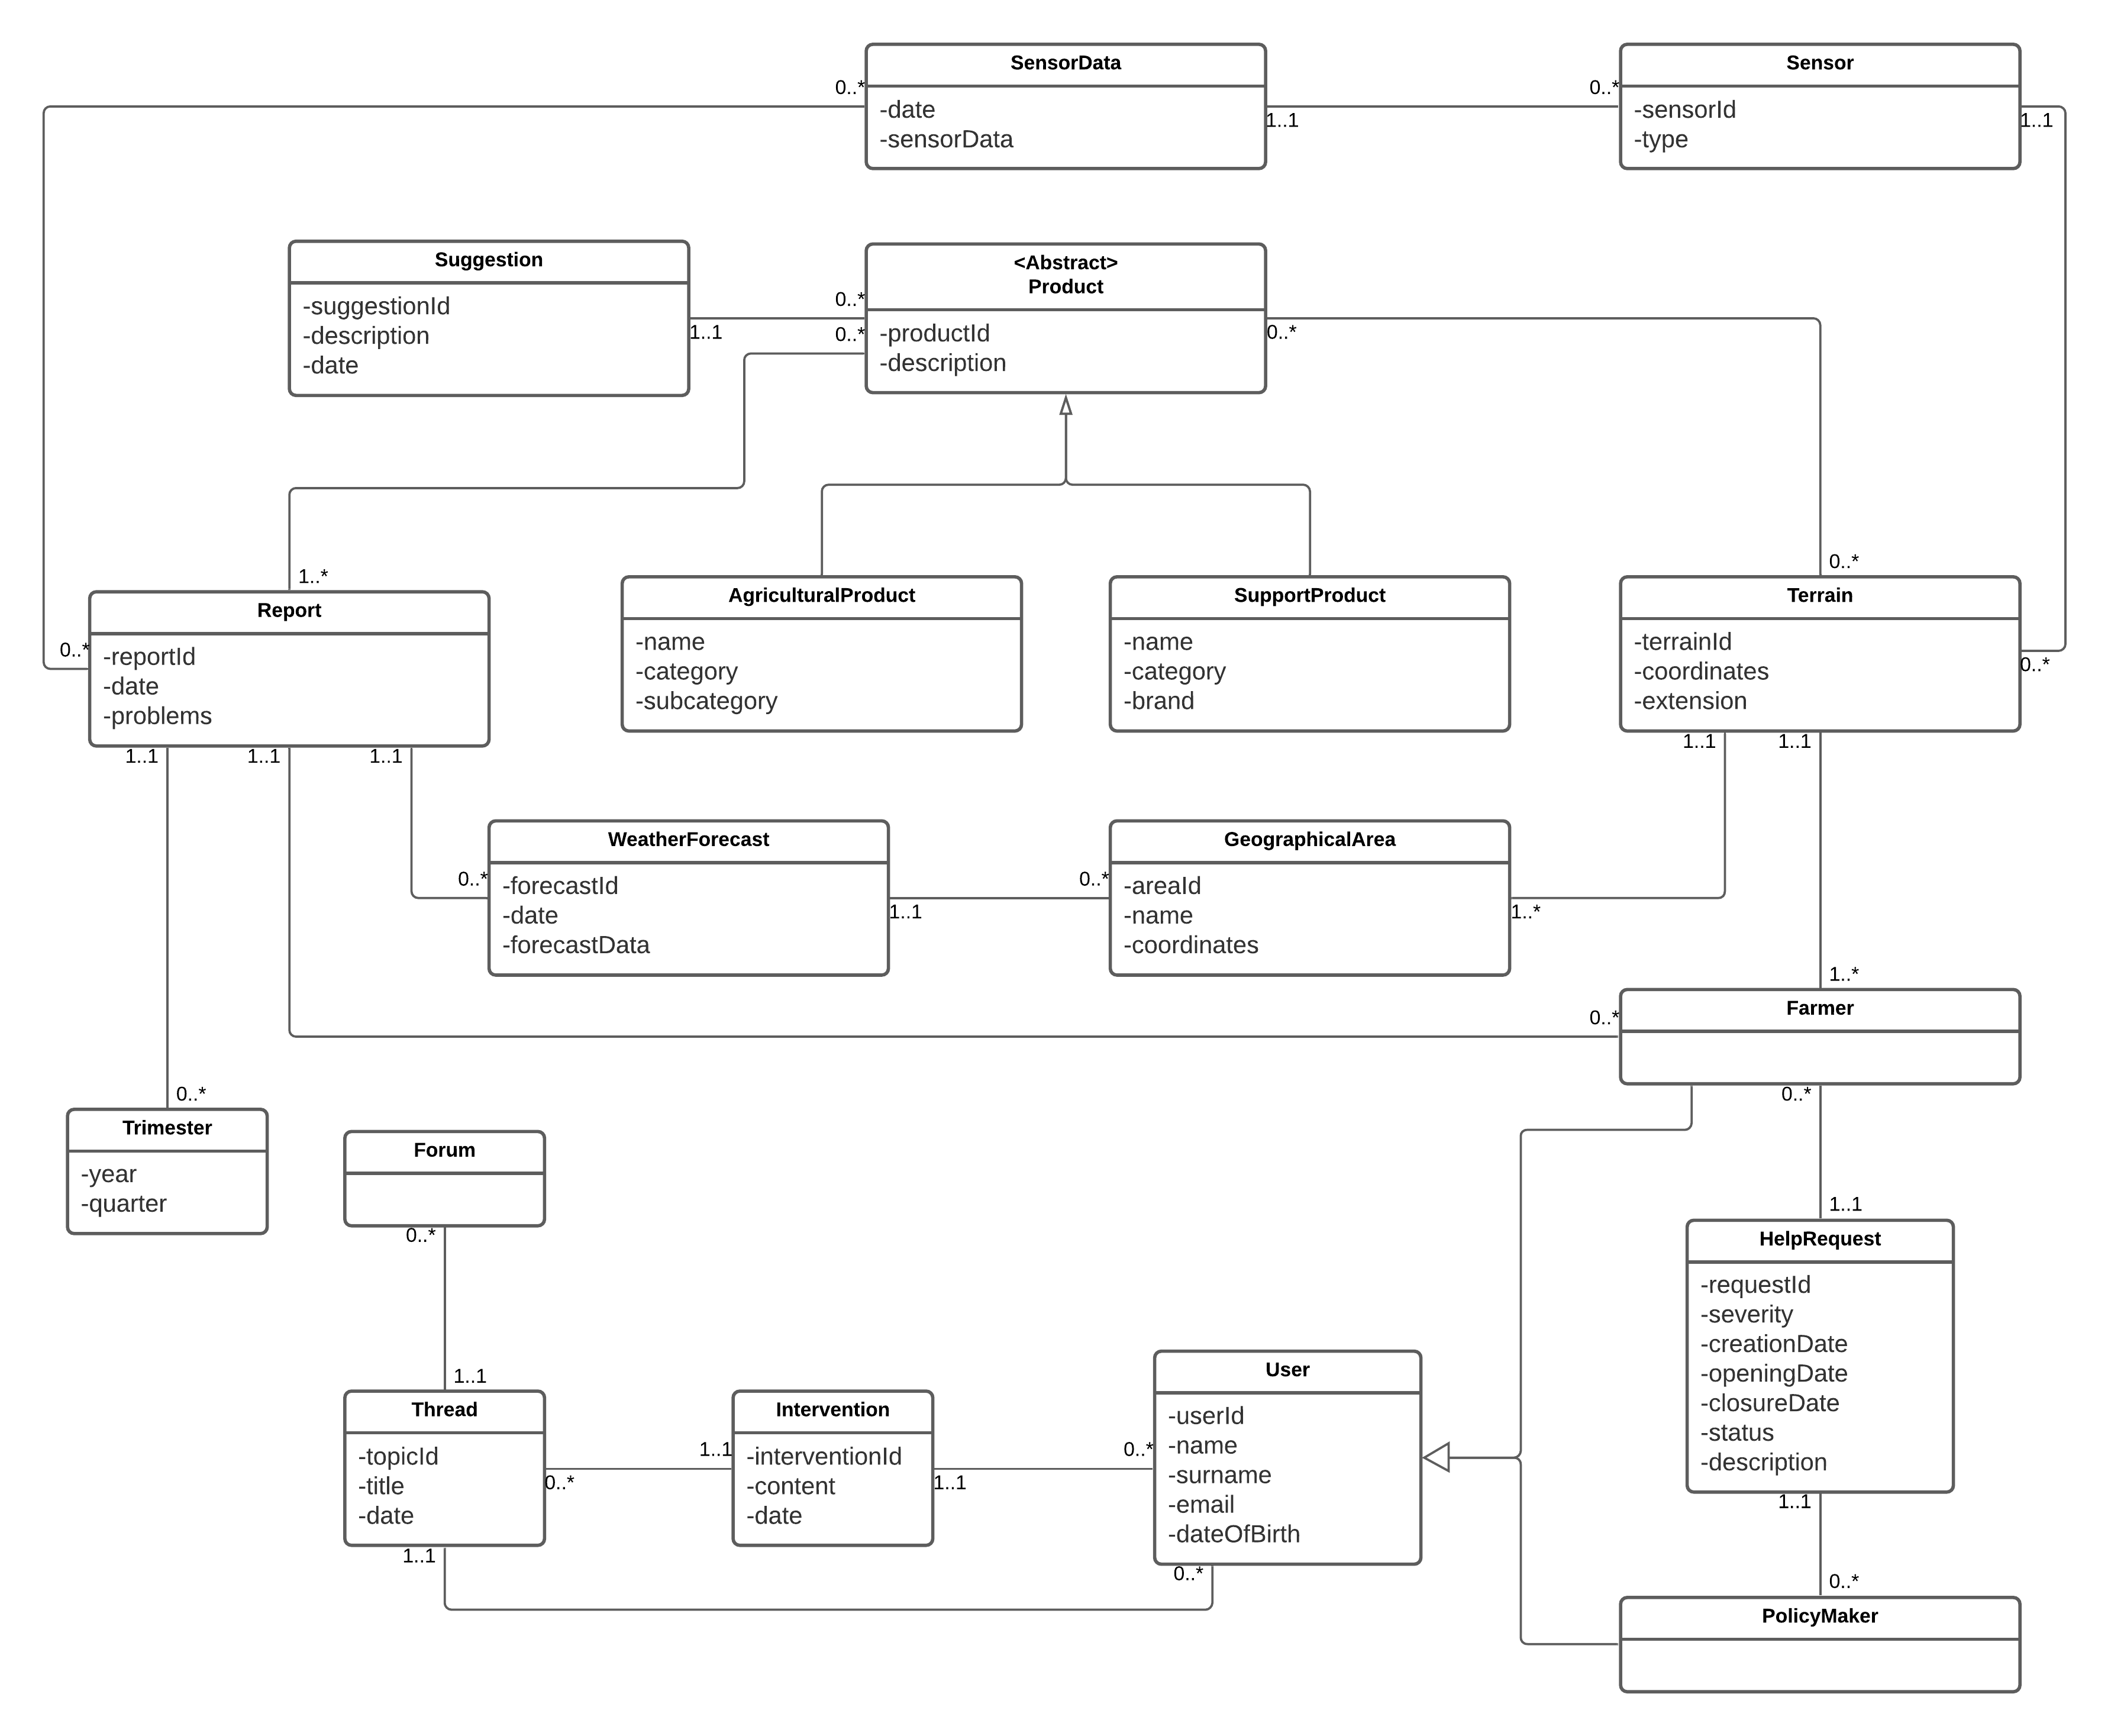
\includegraphics[scale=0.45]{classDiagram.png}
    \caption{Class diagram}
    \label{fig:classDiagram}
\end{figure}
\newpage
\subsubsection{State diagrams}
State diagrams describe the behaviour of the system while considering all possible states the objects can have when an event occurs. This analysis helps to clarify the most critical aspects of the system.
\subsection{Product functions}
This section will summarize the main functionalities of the system.
\subsubsection{Farmers registration}
The procedure of registrating farmers into the system will be supervised by policy makers. Local farmers will not be able to register on their own
but, if they intend to participate to the DREAM project, they will request and be provided with the credentials to login into the system. Policy makers will have to 
register the farmer's anagrafical informations and his possessions according to the local registries. Along with the registration in the system, farmers will be provided with
sensors to facilitate the data gathering process: these sensors will be installed by an expert and they will automatically collect additional information about irrigation that 
will be included in periodical reports.
\subsubsection{Agriculture monitoring}
The system will provide Telangana Policy Makers a platform to monitor and manage the local 
agriculture system. Policy makers will be able to visualize relevant data about goods produced by farmers
and will be able to evaluate their performance based on various parameters. The data will be both inserted manually by farmers
(e.g. data regarding the quantity of goods produced) and automatically collected from sensors (e.g. data regarding weather conditions,
soil humidity and irrigation). The system will automatically process the data to provide policy makers a human-friendly
interface where relevant information will be displayed. The UI will display to TPMs both information obtained through data 
aggregation regarding the overall state of local's agriculture and individual information about farmers performance.
In this way, TPMs will be able to identify farmers whose performance has been particularly good or bad and act on them.
\subsubsection{Farmer's assistance}
The system will provide Telangana's local farmers an easy-to-use platform to obtain relevant information and to favor the interaction with TPMs and other farmers.
Farmers will be able to visualize accurate weather forecasts and personalized suggestions regarding the whole goods production process. They will also be able to 
participate in forum discussions with other farmers, favoring collaboration and exchange of knowledge useful to the collectivity.
DREAM will also provide to farmers an easy way to create help requests and send them to TPMs, in order to facilitate and speed-up the support process and favour
interventions where needed. 
Through DREAM, farmers' performance will be monitored by policy makers, and they will be provided assistance if needed. Also, high-performing farmers will be rewarded
with incentives such as prizes, insurances and invitations to excellence programmes.
\subsubsection{Goods production data insertion and analysis}
In order to monitor and visualize information about the local agricuture system, local farmers participating to the DREAM project 
will be requested to provide the system data regarding their production. Goods production data will then be analyzed and will provide TPMs 
useful informations. 
The collected data will regard:
\begin{itemize}
    \item Quantity of goods produced;
    \item Quantity of products used during the process (e.g. fertilizers);
    \item Quantity of water used in irrigation;
    \item Weather conditions;
    \item Soil humidity
\end{itemize}
The system will then process the collected data, calculating parameters used to evaluate farmers' performance. These parameters include:
\begin{itemize}
    \item Amount of water used based on weather conditions;
    \item Resilience to bad weather;
    \item Ambiental impact of used products;
    \item Crop rotation;
    \item and more %e tanti altri ancora! Scoprili tutti!
\end{itemize}
\subsubsection{Scenarios}
\begin{itemize}
    \item \textit{Registration to the DREAM platform}\\ 
    Santosh is a Telangana's local farmer. He receives a letter from the Ministry of Agriculture, Food and Forestry of Telangana containing information
    about the DREAM project. Santosh thinks that he could benefit from the participation to the programme, so he follows the instructions of the letter and
    sends a application to participate to the DREAM project via e-mail to the Ministry. A few days letter his application is accepted and a policy maker sends him
    via e-mail further instructions: he will be provided with credentials to login into the system and an operator will visit his farm to install sensors to monitor
    irrigation. In the meantime the policy maker inserts into the DREAM database the information about Santosh. When Santosh receives the login credentials, he is 
    ready to access to the system and start participating to the project.
    \item \textit{Insertion of crop collection data into the system.}\\ 
    % specificare anche che il farmer inserisce i problemi che ha affrontato
    Rajesh is a Telangana's local farmer. Every morning he wakes up, does a little and poor breakfast and goes to work in the fields.
    Although being a very humble and physically demanding work, agriculture has always been a priority in Rajesh life: nothing gives him
    more satisfaction than seeing the results of his hard work and when he goes to sleep at night, even though he is tired from the long day of work,
    he falls asleep with a smile on his mouth thinking about his crop happily growing in the night. When the crop is ready to be collected, the atmosphere
    is electric in Rajesh's farm: if the crop is good and particularly abundant, all the workers have a big dinner, finely prepared by Rajesh and his wife,
    followed by a long party night where everybody sings and dances. The day after the celebration, Rajesh wakes up with a tremendous hangover, and proceeds
    to login into the DREAM platform. Once he has logged in, he proceeeds to insert into the system the data regarding the collected crop.
    He would have preferred to sleep a few more hours, and only by looking at the computer's screen he gets a big headache, but he carries on, because he
    remembers that tomorrow will be another happy day in the fields of Telangana.
    \item \textit{Awarding of the best performing farmer}\\
    % Assunzioni che ho fatto: ogni policy maker ha un'area di competenza; ogni trimestre sono selezionati
    % 10 agricoltori in base a degli indici definiti dall'alto; a seguito della chiusura del trimestre il sistema
    % memorizza i dati relativi al semestre appena passato e fa partire l'inizializzazione del nuovo trimestre.
    Guepequesh works as PM at the Ministry of Agriculture, Food and Forestry of Telengana. Like every end of the quarter,
     it's time to designate who the top performing farmers of the period were. Guepequesh logs in with his credentials to
      the DREAM portal and goes to his area of expertise, the dashboard shows the ranking of farmers sorted according to 
      the synthetic indices of interest established by the Committee of Policy Makers of Telengana, updated the same day. 
      Guepequesh selects the top 10 farmers shown in the ranking, sends them an email alert stating that they have been 
      selected as the top performing farmers of the quarter, specifying their position in the ranking. The notice contains 
      instructions on how to claim the prizes they have won, and also indicates the dates available for an interview in which 
      the PM will ask the farmer to provide information about the best practices he uses to grow his crops. After notifying 
      all winners, Guepequesh will notify the system to proceed with the closing of the quarter. In the following days, 
      following the interviews, the PM will enter all data related to the best practices followed by the farmer in the system, 
      and they will be forwarded to all farmers in the area who grow the same type of product. 
      \item \textit{Farmers request for help and suggestions by other farmers}\\
      Marrakesh is a young farmer from Telengana. He has recently decided to strike out on his own in the world of agriculture 
      and knows that he will face many challenges. During a normal day's work, Marrakesh notices that even several hours after irrigation, 
      his soil remains very wet and even puddles form. He had never encountered this problem before and decides to rely on the 
      farmers' forum provided by the DREAM platform to which he is subscribed. Marrakesh logs in and goes to the "Problems and Help Requests" 
      section of the forum, creates a new thread and prepares to fill in the required fields for the submission of the request. 
      The young farmer enters a short title, his working area, the type of shoot with which he encountered the problem and an accurate description 
      of the problem he had. All farmers receive a notification on the platform that a new application has been entered, the notification includes 
      the title and type of sprout so that a farmer can immediately determine if he or she considers themselves competent in the field or not. 
      In particular, an experienced farmer named Rastykilo pauses to read the full description of the problem and enters a very accurate 
      response to the problem. All of the farmers who read the response enter positive feedback, and Marrakesh, the next day, feels confident 
      in following Rastykilo's advice, given the many positive feedbacks.
      \item \textit{Identify those farmers who need to be helped as they are performing particularly badly}
      Om Ashgabash is a Telangana Policy maker. At the end of the trimester, he checks as usual the performances of farmers. He notices that Vidit Parkamush, a local
      farmer of his area of competence, has produced goods for a significantly lower amount than the other farmers over the same periods. He then decides that Vidit might
      need some help in order to perform better in the next period. To help him, first of all he schedules a call with Vidit to understand his situation and evaluate which
      actions might be needed. Once understood the situation, Om decides first of all to provide Vidit some useful suggestions related to his goods production. Then, he adds
      to the local control visits schedule additional visits to Vidit's farm in order to keep under better control his situation for the next months. Vidit is also added to the
      monitoring list, where policy makers can easily check the performances of farmers in difficulty.
\end{itemize}
\subsection{User Characteristics}
In this section the different types of users of the system will be analyzed. DREAM has three categories of users:
\begin{itemize}
    \item \textbf{Farmers}\\
    Telangana Farmers will mainly use the platform to visualize weather forecasts, insert data about goods production, create help requests and intervene
    in forum discussions. It is safe to assume that most of them will not have much familiarity with this kind of procedures and with
    technological products in general. This requires a UI as simple and intuitive as possible, providing them all the desired functionalities
    without requiring much experience with the system. 
    \item \textbf{Policy Makers}\\
    Telangana Policy Makers will use the platform to monitor and manage the local agriculture. They will perform more complex tasks than farmers, such as 
    visualizing data about performance, interact with farmers and manage help requests and suggestions and agronomists' schedules. We can assume that Policy
    Makers will have at least some experience with the use of management software, and they will be provided more complex functionalities that will require 
    some experience and training with the platform.
    \item \textbf{DREAM system admins}\\
    The DREAM platform will also require administration operations from qualified operators. They will have a robust knowledge of the platform since they will 
    perform system's maintenance and update. They will be designed with this role before the deployment of the system and it won't be possible to register to the 
    platform with this role. 
\end{itemize} 
\subsection{Constraints}
This section contains general observations about boundaries that will limit the system options.
\subsubsection{Regulatory policies}
%da pensarne e aggiungerne, poichè siamo pur sempre in un contesto governativo
\subsubsection{Hardware limitations}
The system will have support a broad list of devices since the end users of the product will be likely
to have basic computers with low performances.
\subsubsection{Interfaces to other applications}
DREAM will implement a pre-existing weather forecasting system, which will be integrated via APIs. Failures in the 
system above will not affect the overall functioning of DREAM but will result in wrong forecasts or in the unavailability of the feature.
\subsection{Domain assumptions}
Domain assumptions define the world in which DREAM works. 
\begin{itemize}
    \item[] \textbf{DA1} Each policy maker has one and one only area to monitor.
    \item[] \textbf{DA2} Terrains cannot be shared: each terrain is associate with one and only farmer. 
    \item[] \textbf{DA3} Farmers have a device able to access the platform. 
    \item[] \textbf{DA4} Farmers always insert correct data in the system.
    \item[] \textbf{DA5} Farmers participating to the programme actively use the platform.
    \item[] \textbf{DA6} Farmers' possessions are already registered at the local Ministry.
    \item[] \textbf{DA7} Policy makers' decisions are solely data-driven and are not affected by personal opinions.
    \item[] \textbf{DA8} Humidity soil sensors are already installed and cover the entire geographical area.
    \item[] \textbf{DA9} Each farmer's terrain humidity data is provided by one and only sensor, associated accordingly to geographical distance from the center of the terrain.
    \item[] \textbf{DA10} Data provided by humidity soil sensors is always correct.
    \item[] \textbf{DA11} Each farmer has an automated irrigation system with a control unit.
    \item[] \textbf{DA12} Each irrigation control unit supports the sensors provided by DREAM.
    \item[] \textbf{DA13} Data provided by the irrigation sensors is always correct.
    \item[] \textbf{DA14} The units of measurement used will always be consistent. 
\end{itemize}
\newpage
\section{Specific Requirements}
\subsection{External Interface Requirements}
\subsubsection{User Interfaces}
    \begin{figure}[h]
    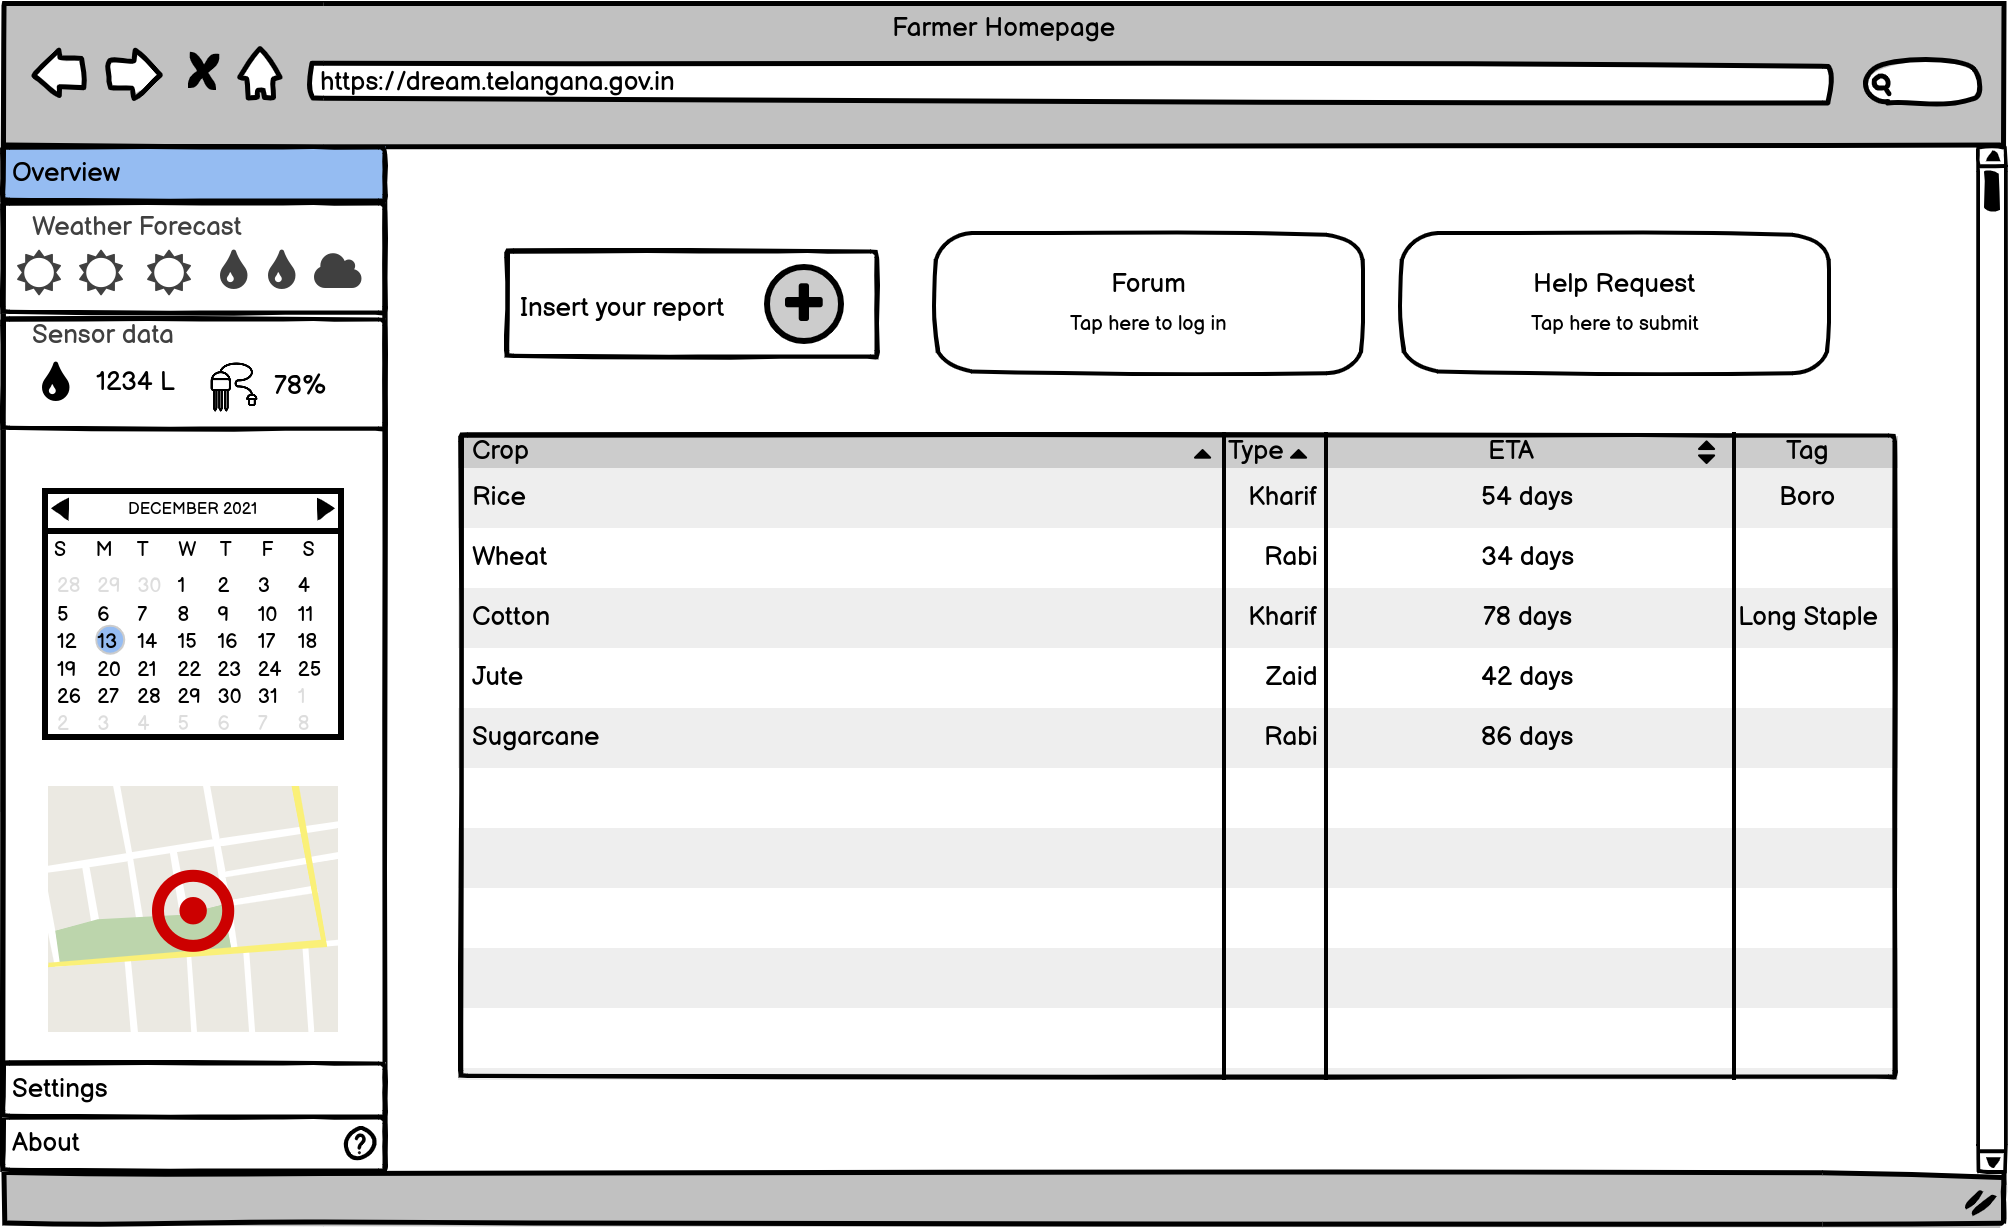
\includegraphics[width=14cm]{farmer_homepage.png} 
    \caption{Homepage of farmer's web application} 
    \end{figure}
    \newpage
    \begin{figure}[ht]
    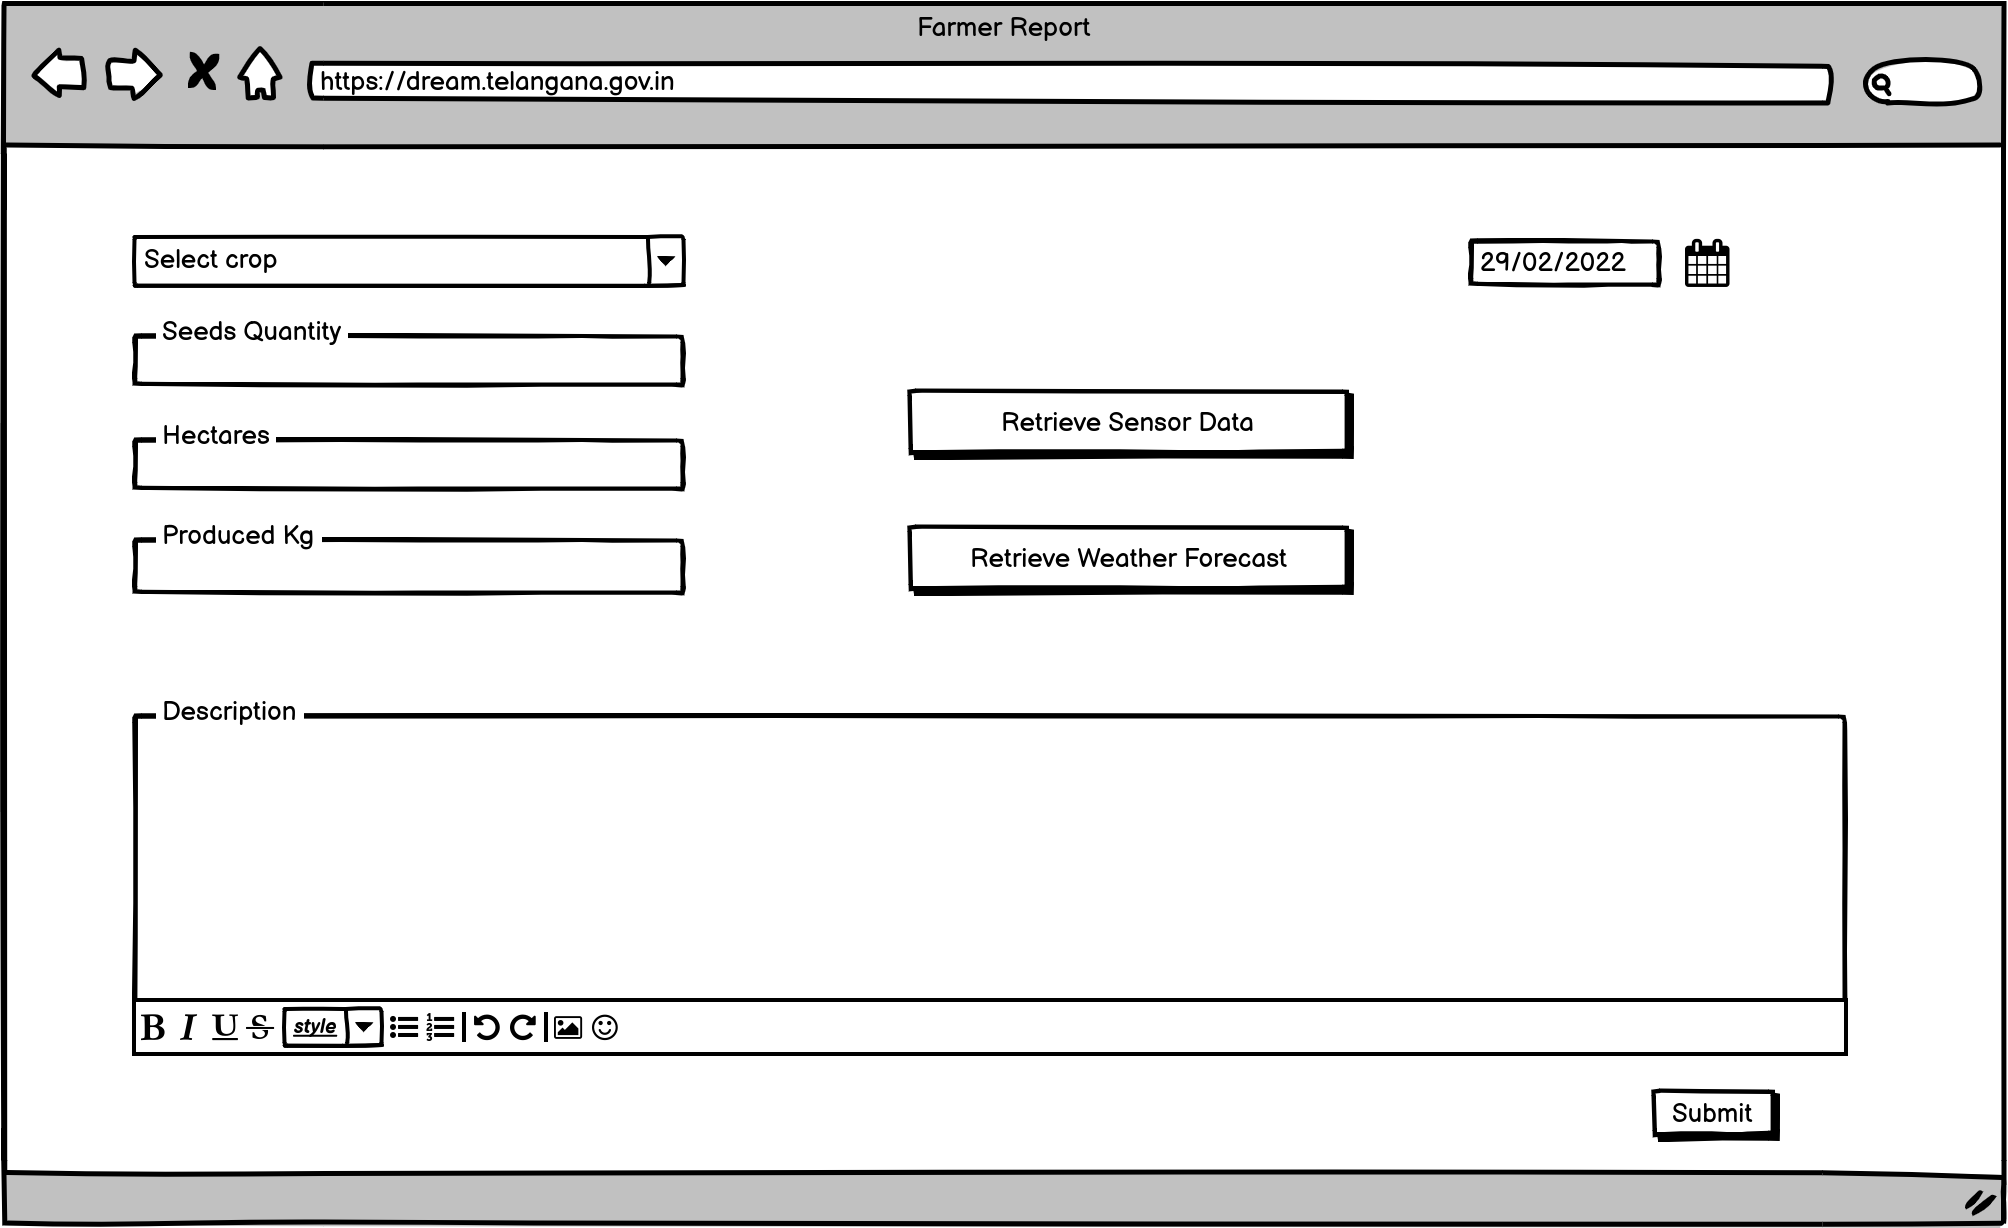
\includegraphics[width=14cm]{report.png}  
    \caption{Farmer report form page}
    \end{figure}
\begin{figure}[ht!]
    \centering
    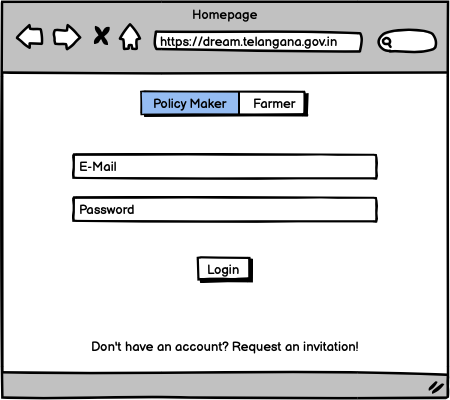
\includegraphics[scale=0.45]{ui/login.png}
    \caption{Login page}
\end{figure}
\begin{figure}[ht!]
    \centering
    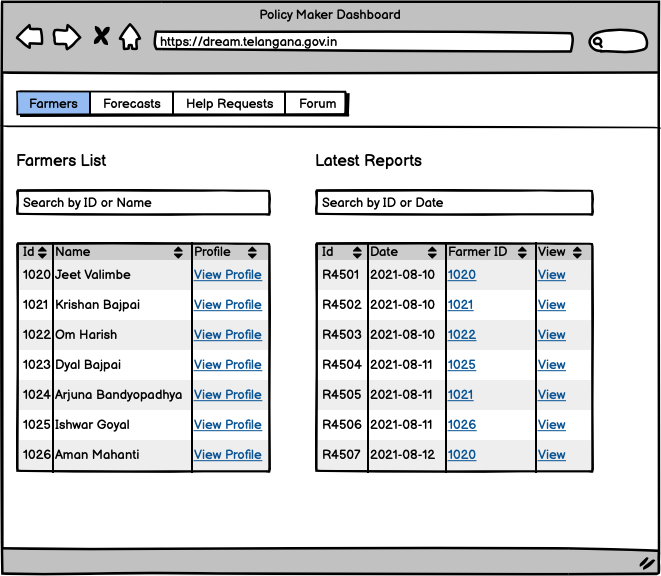
\includegraphics[scale=0.30]{ui/pm_farmers.png}
    \caption{PM Dashboard - Farmers page}
\end{figure}
\begin{figure}[ht!]
    \centering
    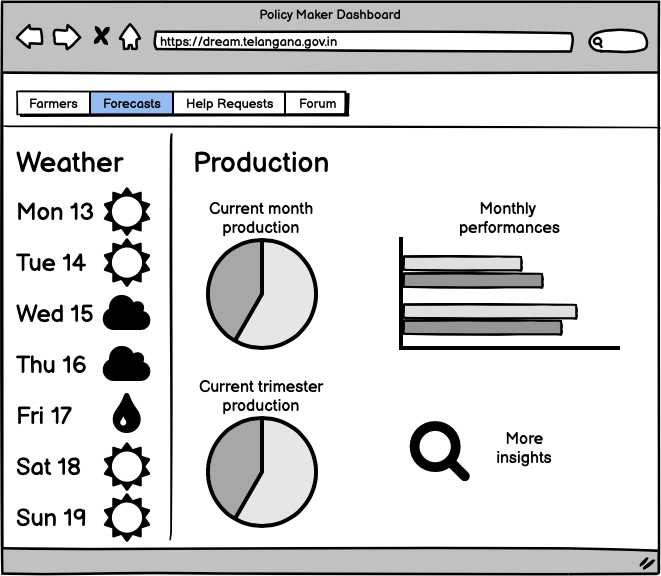
\includegraphics[scale=0.40]{ui/pm_forecasts.png}
    \caption{PM Dashboard - Forecasts page}
\end{figure}
\begin{figure}[ht!]
    \centering
    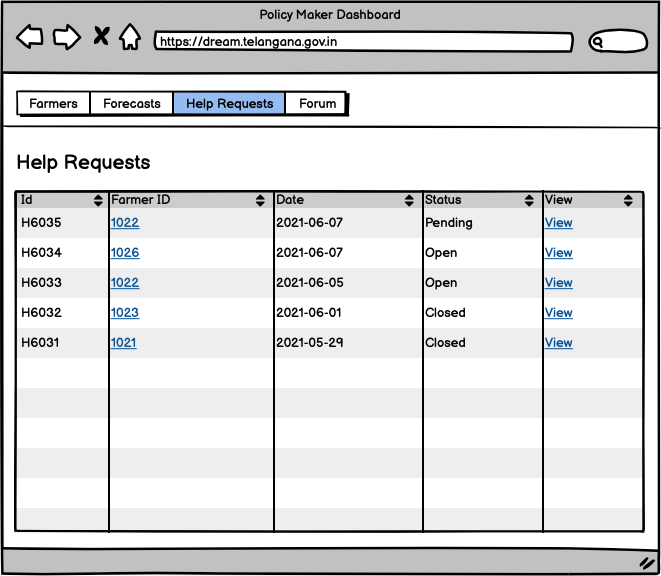
\includegraphics[scale=0.40]{ui/pm_helprequests.png}
    \caption{PM Dashboard - Help Requests page}
\end{figure}
\begin{figure}[ht!]
    \centering
    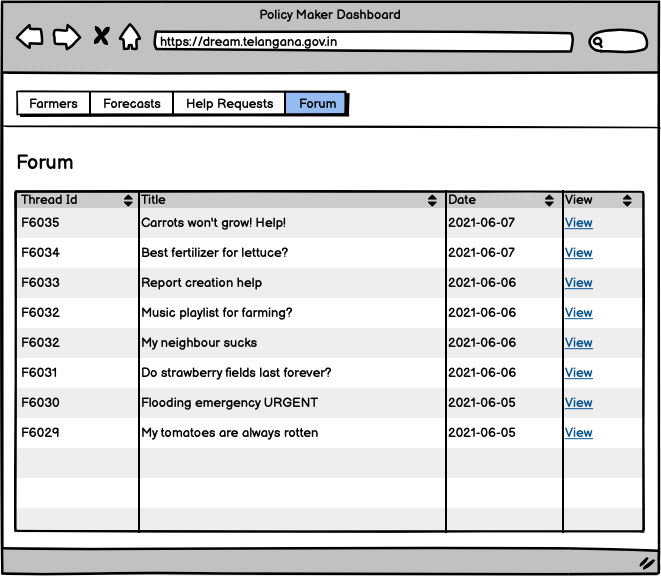
\includegraphics[scale=0.40]{ui/pm_forum.png}
    \caption{PM Dashboard - Forum page}
\end{figure}
\begin{figure}[ht!]
    \centering
    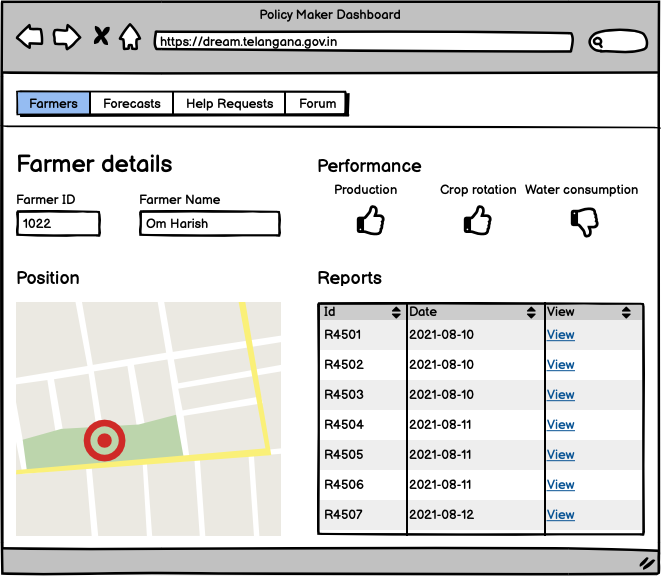
\includegraphics[scale=0.40]{ui/pm_farmerdetail.png}
    \caption{PM Dashboard - Farmer detail page}
\end{figure}
\begin{figure}[ht!]
    \centering
    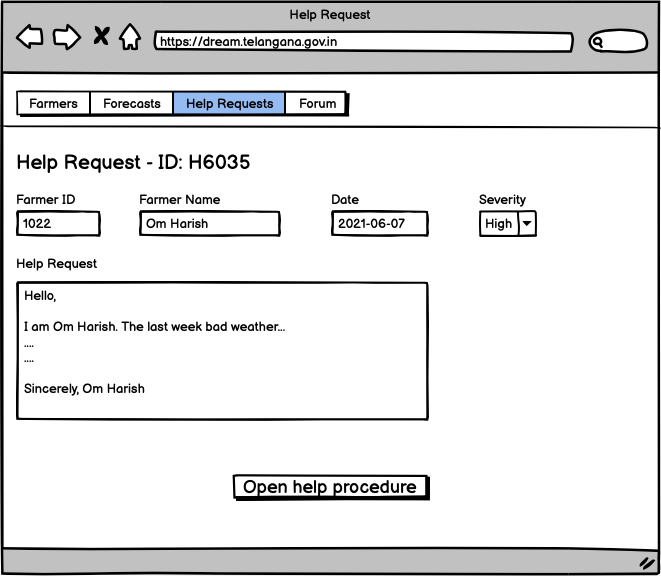
\includegraphics[scale=0.40]{ui/pm_helpdetail.png}
    \caption{PM Dashboard - Help request detail page}
\end{figure}
\begin{figure}[ht!]
    \centering
    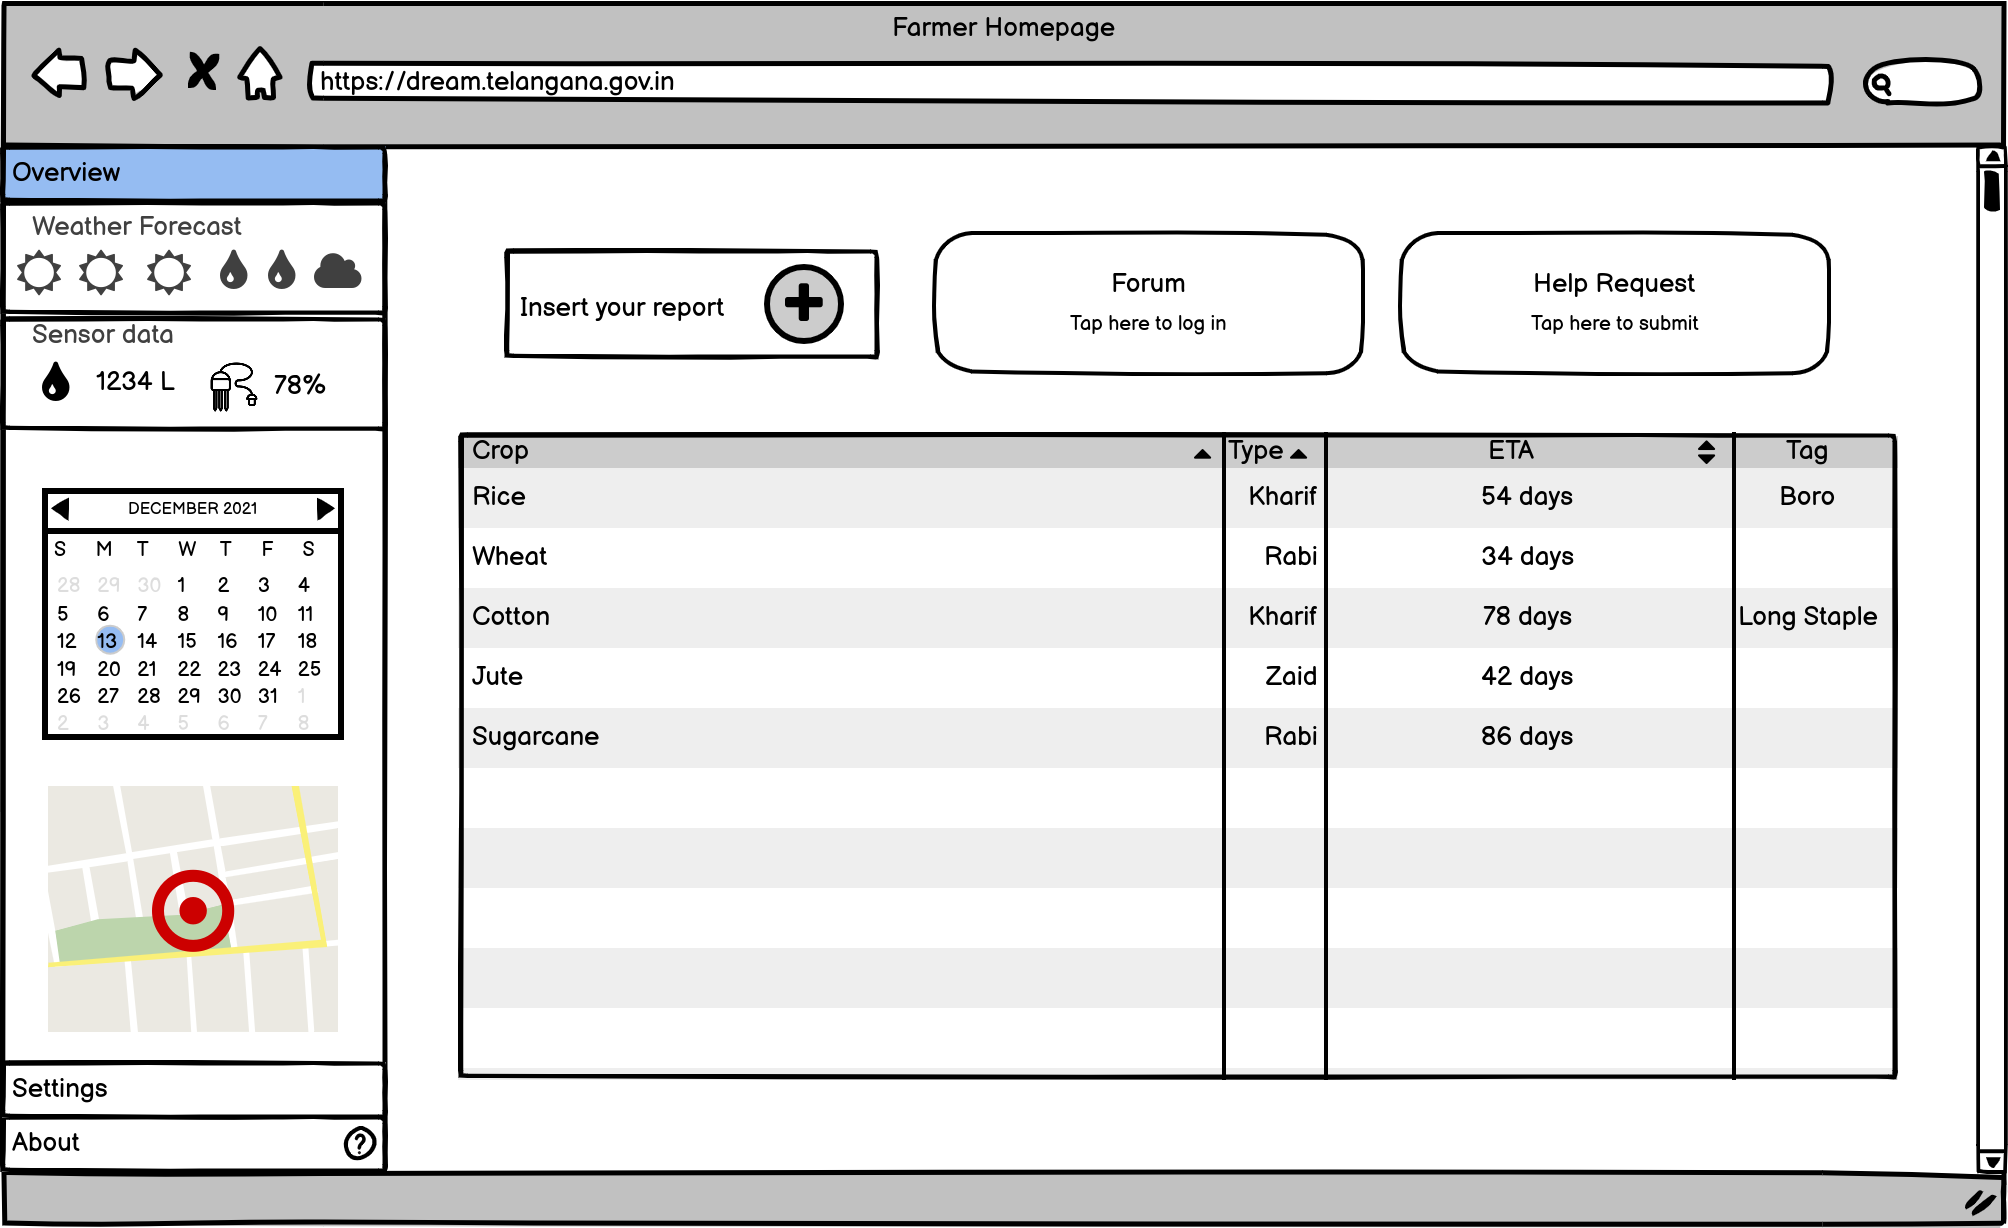
\includegraphics[scale=0.15]{ui/f_homepage.png}
    \caption{Farmer Dashboard - Homepage}
\end{figure}
\newpage
\subsubsection{Hardware Interfaces}
% https://iopscience.iop.org/article/10.1088/1742-6596/1339/1/012012/meta se citiamo anche degli articoli accademici è una bella flexata
Different types of hardware interfaces will be required to ensure that the entire infrastructure functions properly.\\
Farmers and PMs will need to have computers connected to the internet and capable of supporting DREAM's dedicated web app.\\
All sensors will have to use IoT technologies, in fact they will necessarily have to be connected to a Wi-Fi module and programmed to create data and send it to the DREAM server. 
\subsubsection{Software Interfaces}
The system will use the external API of the Telengana governmental weather service to collect and transmit data of interest to farmers, depending on their area.\\
The system doesn't provide any API to external application because of the privacy of the farmers.
\subsubsection{Communication Interfaces}
All the communications between end-devices and the central system are made via internet using the HTTPS protocol.
The communications between clients and sensors are made via a publish-subscribe communication protocol, namely MQTT.
\subsection{Functional Requirements}
\subsubsection{Requirements}
\begin{enumerate}[label=\textbf{R\arabic*}]
    \item \label{req:pmReg} The system shall allow system admins to register policy maker.    
    \item \label{req:pmLogin} The system shall allow policy makers to login.    
    \item \label{req:farmerReg1} The system shall allow policy makers to register farmers.    
    \item \label{req:farmerCreds} The system shall provide farmers credentials to log in.    
    \item \label{req:farmerReg2} The system shall allow farmers to complete their profile information.    
    \item \label{req:farmerLogin} The system shall allow farmers to log into the platform.      
    \item \label{req:farmerReport1} The system shall allow farmers to fill reports with data about goods production.    
    \item \label{req:farmerReport2} The system shall allow farmers to fill reports with data about auxiliary products used for goods production.    
    \item \label{req:farmerReport3} The system shall allow farmers to fill reports with problems faced during goods production.     
    \item \label{req:farmerReport4} The system shall retrieve data from sensors and attach it to reports.     
    \item \label{req:farmerReport5} The system shall retrieve data from weather stations and attach it to reports.     
    \item \label{req:farmerWeather} The system shall allow farmers to visualize weather forecasts.
    \item \label{req:farmerSensors} The system shall allow farmers to visualize data retrieved from humidity and irrigation sensors.
    \item \label{req:farmerForum} The system shall allow farmers to create and contribute to forum discussions.    
    \item \label{req:farmerHelp} The system shall allow farmers to create help requests.     
    \item \label{req:farmerSugg} The system shall allow farmers to visualize personalized suggestions about goods and techniques.    
    \item \label{req:pmMonitor} The system shall allow PMs to monitor farmers' performances.    
    \item \label{req:pmParameters} The system shall provide PMs with parameters to evaluate farmers' performances.   
    \item \label{req:pmGrades} The system shall allow PMs to compare and aggregate farmers' performances.    
    \item \label{req:pmFilter1} The system shall allow PMs to filter farmers based on their information.    
    \item \label{req:pmFilter2} The system shall allow PMs to filter farmers based on their performance.    
    \item \label{req:pmSort1} The system shall allow PMs to sort farmers based on their information.    
    \item \label{req:pmSort2} The system shall allow PMs to sort farmers based on their performance.     
    \item \label{req:pmRewards} The system shall allow PMs to reward best performing farmers.    
    \item \label{req:pmWeather} The system shall allow PMs to visualize weather forecasts.    
    \item \label{req:pmHelp1} The system shall allow PMs to visualize help requests.
    \item \label{req:pmHelp2} The system shall allow PMs to take charge of help requests.
    \item \label{req:pmHelp3} The system shall allow PMs to visualize farmers who have requested help and their performances.
    \item \label{req:pmHelp4} The system shall allow PMs to close help requests.
    \item \label{req:pmInterview} The system shall allow PMs to file reports about farmers interviews.    
    \item \label{req:pmVisits} The system shall allow PMs to re-schedule agronommist's control visit plans.    
    \item \label{req:pmForum} The system shall allow PMs to create and contribute to forum discussions.    
    \item \label{req:pmSuggestions} The system shall allow PMs to create suggestions.
\end{enumerate}
\subsubsection{Goal Mapping on Requirements}
\begin{description}
    \item \textbf{G1 Allow Telangana's Policy Makers to monitor local agriculture}
        \begin{description}
            \item \ref{req:pmReg}\ The system shall allow system admins to register policy maker.
            \item \ref{req:pmLogin} The system shall allow policy makers to login.
            \item \ref{req:pmMonitor} The system shall allow PMs to monitor farmers' performances.
            \item \ref{req:pmParameters} The system shall provide PMs with parameters to evaluate farmers' performances.
            \item \ref{req:pmGrades} The system shall allow PMs to compare and aggregate farmers' performances.
            \item \ref{req:pmFilter1} The system shall allow PMs to filter farmers based on their information.
            \item \ref{req:pmFilter2} The system shall allow PMs to filter farmers based on their performance.
            \item \ref{req:pmSort1} The system shall allow PMs to sort farmers based on their information.
            \item \ref{req:pmSort2} The system shall allow PMs to sort farmers based on their performance.
            \item \ref{req:pmWeather} The system shall allow PMs to visualize weather forecasts.
        \end{description}
    \item \textbf{G2 Allow farmers to receive assistance or rewards based on their performance}
        \begin{description}
            \item \ref{req:farmerReg1} The system shall allow policy makers to register farmers.    
            \item \ref{req:farmerCreds} The system shall provide farmers with credentials to log in.
            \item \ref{req:farmerReg2} The system shall allow farmers to complete their profile information.
            \item \ref{req:farmerLogin} The system shall allow farmers to log into the platform.
            \item \ref{req:farmerReport1} The system shall allow farmers to fill reports with data about goods production.
            \item \ref{req:farmerReport2} The system shall allow farmers to fill reports with data about auxiliary products used for goods production.
            \item \ref{req:farmerReport3} The system shall allow farmers to fill reports with problems faced during goods production.
            \item \ref{req:farmerReport4} The system shall retrieve data from sensors and attach it to reports.
            \item \ref{req:farmerReport5} The system shall retrieve data from weather stations and attach it to reports.
            \item \ref{req:pmRewards} The system shall allow PMs to reward best performing farmers.
            \item \ref{req:pmInterview} The system shall allow PMs to file reports about farmers interviews.
            \item \ref{req:pmVisits} The system shall allow PMs to re-schedule agronommist's control visit plans.
        \end{description}
    \item \textbf{G3 Allow farmers to request and receive help}
        \begin{description}
            \item \ref{req:farmerReg1} The system shall allow policy makers to register farmers.    
            \item \ref{req:farmerCreds} The system shall provide farmers with credentials to log in.    
            \item \ref{req:farmerReg2} The system shall allow farmers to complete their profile information.    
            \item \ref{req:farmerLogin} The system shall allow farmers to log into the platform.
            \item \ref{req:farmerHelp} The system shall allow farmers to create help requests.     
            \item \ref{req:farmerSugg} The system shall allow farmers to visualize personalized suggestions about goods and techniques. 
            \item \ref{req:pmHelp1} The system shall allow PMs to visualize help requests.
            \item \ref{req:pmHelp2} The system shall allow PMs to take charge of help requests.
            \item \ref{req:pmHelp3} The system shall allow PMs to visualize farmers who have requested help and their performances.
            \item \ref{req:pmHelp4} The system shall allow PMs to close help requests.
            \item \ref{req:pmSuggestions} The system shall allow PMs to create suggestions.
        \end{description}
    \item \textbf{G4 Create a farmer's network to promote collaboration and mutual aid}
        \begin{description}
            \item \ref{req:farmerReg1} The system shall allow policy makers to register farmers.    
            \item \ref{req:farmerCreds} The system shall provide farmers with credentials to log in.    
            \item \ref{req:farmerReg2} The system shall allow farmers to complete their profile information.    
            \item \ref{req:farmerLogin} The system shall allow farmers to log into the platform.
            \item \ref{req:farmerForum} The system shall allow farmers to create and contribute to forum discussions.
            \item \ref{req:pmForum} The system shall allow PMs to create and contribute to forum discussions.
        \end{description}
        \item \textbf{G5 Improve farmer's productivity}
        \begin{description}
            \item \ref{req:farmerReg1} The system shall allow policy makers to register farmers.    
            \item \ref{req:farmerCreds} The system shall provide farmers with credentials to log in.    
            \item \ref{req:farmerReg2} The system shall allow farmers to complete their profile information.    
            \item \ref{req:farmerLogin} The system shall allow farmers to log into the platform.
            \item \ref{req:farmerWeather} The system shall allow farmers to visualize weather forecasts.
            \item \ref{req:farmerSensors} The system shall allow farmers to visualize data retrieved from humidity and irrigation sensors.
            \item \ref{req:farmerHelp} The system shall allow farmers to create help requests.     
            \item \ref{req:farmerSugg} The system shall allow farmers to visualize personalized suggestions about goods and techniques.
            \item \ref{req:pmSuggestions} The system shall allow PMs to create suggestions.
        \end{description}
\end{description}
\newpage
\subsubsection{Use Cases}
\begin{enumerate}[label=\textbf{UC\arabic*}]
    \item \label{uc:uc1} \textbf{Policy maker registration}
        \begin{longtable}{p{0.26\linewidth}p{0.75\linewidth}}
            \toprule
            \textbf{Name} & \textbf{Policy maker registration} \\
            \midrule
            \textbf{Actors} & System admin, Policy Maker\\
            \midrule
            \textbf{Entry conditions} &
            \begin{itemize}
                \item The platform is running
                \item The system admin has logged into the system
            \end{itemize}\\
            \midrule
            \textbf{Flow of events} & 
            \begin{enumerate}
                \item The system admin creates a new policy maker profile
                \item The system admin inserts the policy maker data in the newly created profile
                \item The system automatically generates log in credentials for the policy maker
                \item The system automatically sends an e-mail to the address associated to the profile containing credentials and instructions to log in
            \end{enumerate} \\
            \midrule
            \textbf{Exit conditions} & The policy maker receives his credentials\\
            \midrule
            \textbf{Exceptions} & 
            \begin{itemize}
                \item If the policy maker e-mail address is already in use, the process is aborted.
            \end{itemize} \\
            \bottomrule
            \caption{\emph{Policy maker registration} use case description}
        \end{longtable}
    \newpage
    \item \label{uc:uc2} \textbf{Farmer Registration} 
        \begin{longtable}{p{0.26\linewidth}p{0.75\linewidth}}
            \toprule
            \textbf{Name} & \textbf{Farmer Registration} \\
            \midrule
            \textbf{Actors} & Farmer, Policy Maker \\
            \midrule
            \textbf{Entry conditions} & 
            \begin{itemize}
                \item The platform is running
                \item The policy maker has logged into the system
            \end{itemize}\\
            \midrule
            \textbf{Flow of events} & 
            \begin{enumerate}
                \item The policy maker sends an invite via e-mail to the farmer
                \item The farmer accepts the invite 
                \item The policy maker creates a new profile and inserts the farmer data
                \item The system generates the credentials for the farmer login
                \item The farmer receives the credentials via e-mail
                \item The farmer logs into the platform and completes the registration
                \item The system saves the farmer data
            \end{enumerate} \\
            \midrule
            \textbf{Exit conditions} & The farmer is registered in the system\\
            \midrule
            \textbf{Exceptions} & 
            \begin{itemize}
                \item If the farmer does not complete the registration in time, the process is aborted. The farmer can request to repeat the registration by sending an e-mail.
            \end{itemize} \\
            \bottomrule
            \caption{\emph{Farmer Registration} use case description}
        \end{longtable}
    \newpage
    \item \label{uc:uc3} \textbf{User login} 
    \begin{longtable}{p{0.26\linewidth}p{0.75\linewidth}}
        \toprule
        \textbf{Name} & \textbf{Farmer Registration} \\
        \midrule
        \textbf{Actors} & Farmer, Policy Maker \\
        \midrule
        \textbf{Entry conditions} & The platform is running \\
        \midrule
        \textbf{Flow of events} & 
        \begin{enumerate}
            \item The user goes to the login page
            \item The user inserts the login credentials
            \item The user submits the form
        \end{enumerate} \\
        \midrule
        \textbf{Exit conditions} & The user has successfully logged into the platform\\
        \midrule
        \textbf{Exceptions} & 
        \begin{itemize}
            \item If the login credentials are incorrect, the system notifies the user and the process is aborted.
        \end{itemize} \\
        \bottomrule
        \caption{\emph{Farmer Registration} use case description}
    \end{longtable}
    \newpage
    \item \label{uc:uc4} \textbf{Insertion of report}
        \begin{longtable}{p{0.26\linewidth}p{0.75\linewidth}}
            \toprule
            \textbf{Name} & \textbf{Insertion of report} \\
            \midrule
            \textbf{Actors} & Farmer\\
            \midrule
            \textbf{Entry conditions} & 
            \begin{itemize}
                \item The platform is running
                \item The farmer has logged into the system
                \item The farmer has collected his crop
            \end{itemize}\\
            \midrule
            \textbf{Flow of events} & 
            \begin{enumerate}
                \item The farmer inserts the type and quantity of goods produced
                \item The farmer inserts the type and quantity of support products used
                \item The farmer application retrieves data from sensors and inserts it into the report
                \item The farmer sends the report
                \item The system checks the report
                \item The system stores the report
            \end{enumerate} \\
            \midrule
            \textbf{Exit conditions} & The report is stored in the system\\
            \midrule
            \textbf{Exceptions} & 
            \begin{itemize}
                \item If the report contains wrong information, the process is aborted.
            \end{itemize} \\
            \bottomrule
            \caption{\emph{Insertion of report} use case description}
        \end{longtable}
    \newpage
    \item \label{uc:uc5} \textbf{Creation and handling of a help request}
        \begin{longtable}{p{0.26\linewidth}p{0.75\linewidth}}
            \toprule
            \textbf{Name} & \textbf{Creation and handling of a help request} \\
            \midrule
            \textbf{Actors} & Farmer, Policy Maker\\
            \midrule
            \textbf{Entry conditions} & 
            \begin{itemize}
                \item The platform is running
                \item The farmer has logged into the system
                \item The policy maker has logged into the system
                \item The farmer needs help
            \end{itemize}\\
            \midrule
            \textbf{Flow of events} & 
            \begin{enumerate}
                \item The farmer compiles the help request form
                \item The help request is created with \textit{pending} status
                \item The policy maker takes charge of the help request
                \item The help request status becomes \textit{open}
                \item The policy maker evaluates the severity of the help request
                \item The policy maker takes the necessary actions based on the severity
                \item The policy maker monitors the farmer's performances in the next period
                \item If the farmer's performances do not improve, the severity of the request is increased and new actions are taken (\textit{back to (f)})
                \item If the farmer's performances improve, the help request is closed 
            \end{enumerate} \\
            \midrule
            \textbf{Exit conditions} & The help request status becomes \textit{closed}\\
            \midrule
            \textbf{Exceptions} & 
            \begin{itemize}
                \item The farmer can close the help request by itself during the process if authority help is no more necessary
            \end{itemize} \\
            \bottomrule
            \caption{\emph{Creation and handling of a help request} use case description}
        \end{longtable}
    \newpage
    \item \label{uc:uc6} \textbf{Interview of a good-performing farmer}
        \begin{longtable}{p{0.26\linewidth}p{0.75\linewidth}}
            \toprule
            \textbf{Name} & \textbf{Interview of a good-performing farmer} \\
            \midrule
            \textbf{Actors} & Farmer, Policy Maker\\
            \midrule
            \textbf{Entry conditions} & 
            \begin{itemize}
                \item The platform is running
                \item The policy maker has logged into the system
                \item The policy maker identifies a good-performing farmer
            \end{itemize}\\
            \midrule
            \textbf{Flow of events} & 
            \begin{enumerate}
                \item The policy maker sends a request for an interview to the selected farmer
                \item The farmer responds to the request
                \item If the response is negative, the process is aborted
                \item If the response is positive, the policy maker and the farmer agree on a date to do the interview
                \item On the decided date, an interview via phone is held
                \item Once the interview is ended, the policy maker inserts into the system the relevant information obtained (e.g. suggestions to other farmers)
            \end{enumerate} \\
            \midrule
            \textbf{Exit conditions} & The interview information is inserted into the system\\
            \midrule
            \textbf{Exceptions} & 
            \begin{itemize}
                \item If the policy maker and the farmer cannot agree on a date, the process is aborted
            \end{itemize} \\
            \bottomrule
            \caption{\emph{Interview of a good-performing farmer} use case description}
        \end{longtable}
    \newpage
    \item \label{uc:uc7} \textbf{Rewarding of good-performing farmers}
        \begin{longtable}{p{0.26\linewidth}p{0.75\linewidth}}
            \toprule
            \textbf{Name} & \textbf{Rewarding of good-performing farmers} \\
            \midrule
            \textbf{Actors} & Farmer, Policy Maker\\
            \midrule
            \textbf{Entry conditions} & 
            \begin{itemize}
                \item The platform is running
                \item The policy maker has logged into the system
                \item The trimester has ended
            \end{itemize}\\
            \midrule
            \textbf{Flow of events} & 
            \begin{enumerate}
                \item The policy maker visualizes the list of the top 10 performing farmers of the trimester
                \item The PM sends to each of them a mail notificating that their performances were excellent and containing instructions on how to claim their rewards
                \item For each farmer, an interview is scheduled (if possible)
            \end{enumerate} \\
            \midrule
            \textbf{Exit conditions} & Every interview is scheduled\\
            \midrule
            \bottomrule
            \caption{\emph{Rewarding of good-performing farmers} use case description}
        \end{longtable}
    \newpage
\end{enumerate}
\subsubsection{Traceability matrix}
\begin{table}[]
    \begin{tabular}{c|ccccc|cccccccc}
        & \ref{goal:g1} & \ref{goal:g2} & \ref{goal:g3} & \ref{goal:g4} & \ref{goal:g5} & \ref{uc:uc1} & \ref{uc:uc2} & \ref{uc:uc3} & \ref{uc:uc4} & \ref{uc:uc5} & \ref{uc:uc6} & \ref{uc:uc7} & UC8 \\ \hline
    \ref{req:pmReg}  & X &  &  &  &  & X &  &  &  &  &  &  &  \\
    \ref{req:pmLogin}  & X &  &  &  &  &  &  & X &  & X & X & X &  \\
    \ref{req:farmerReg1}  &  & X & X & X & X &  & X &  &  &  &  &  &  \\
    \ref{req:farmerCreds}  &  & X & X & X & X &  & X &  &  &  &  &  &  \\
    \ref{req:farmerReg2}  &  & X & X & X & X &  & X &  &  &  &  &  &  \\
    \ref{req:farmerLogin}  &  & X & X & X & X &  &  & X & X & X & X & X & X \\
    \ref{req:farmerReport1}  &  & X &  &  &  &  &  &  & X &  &  &  &  \\
    \ref{req:farmerReport2}  &  & X &  &  &  &  &  &  & X &  &  &  &  \\
    \ref{req:farmerReport3}  &  & X &  &  &  &  &  &  & X &  &  &  &  \\
    \ref{req:farmerReport4}  &  & X &  &  &  &  &  &  & X &  &  &  &  \\
    \ref{req:farmerReport5}  &  & X &  &  &  &  &  &  & X &  &  &  &  \\
    \ref{req:farmerWeather}  &  &  &  &  & X &  &  &  &  & X &  &  &  \\
    \ref{req:farmerSensors}  &  &  &  &  & X &  &  &  &  & X &  &  &  \\
    \ref{req:farmerForum}  &  &  &  & X &  &  &  &  &  &  &  &  & X \\
    \ref{req:farmerHelp}  &  &  & X &  & X &  &  &  &  & X &  &  &  \\
    \ref{req:farmerSugg}  &  &  & X &  & X &  &  &  &  & X &  &  &  \\
    \ref{req:pmMonitor}  & X &  &  &  &  &  &  &  &  &  &  & X &  \\
    \ref{req:pmParameters}  & X &  &  &  &  &  &  &  &  &  &  & X &  \\
    \ref{req:pmGrades}  & X &  &  &  &  &  &  &  &  &  &  & X &  \\
    \ref{req:pmFilter1}  & X &  &  &  &  &  &  &  &  &  &  & X &  \\
    \ref{req:pmFilter2}  & X &  &  &  &  &  &  &  &  &  &  & X &  \\
    \ref{req:pmSort1}  & X &  &  &  &  &  &  &  &  &  &  & X &  \\
    \ref{req:pmSort2}  & X &  &  &  &  &  &  &  &  &  &  & X &  \\
    \ref{req:pmRewards}  &  & X &  &  &  &  &  &  &  &  &  & X &  \\
    \ref{req:pmWeather}  & X &  &  &  &  &  &  &  &  & X &  &  &  \\
    \ref{req:pmHelp1}  &  &  & X &  &  &  &  &  &  & X &  &  &  \\
    \ref{req:pmHelp2}  &  &  & X &  &  &  &  &  &  & X &  &  &  \\
    \ref{req:pmHelp3}  &  &  & X &  &  &  &  &  &  & X &  &  &  \\
    \ref{req:pmHelp4}  &  &  & X &  &  &  &  &  &  & X &  &  &  \\
    \ref{req:pmInterview}  &  & X &  &  &  &  &  &  &  &  & X & X &  \\
    \ref{req:pmVisits}  &  & X &  &  &  &  &  &  &  &  & X & X &  \\
    \ref{req:pmForum}  &  &  &  & X &  &  &  &  &  &  &  &  & X \\
    \ref{req:pmSuggestions}  &  &  & X &  & X &  &  &  &  & X &  &  &  \\
    \end{tabular}
\end{table}
\begin{figure}[h]
    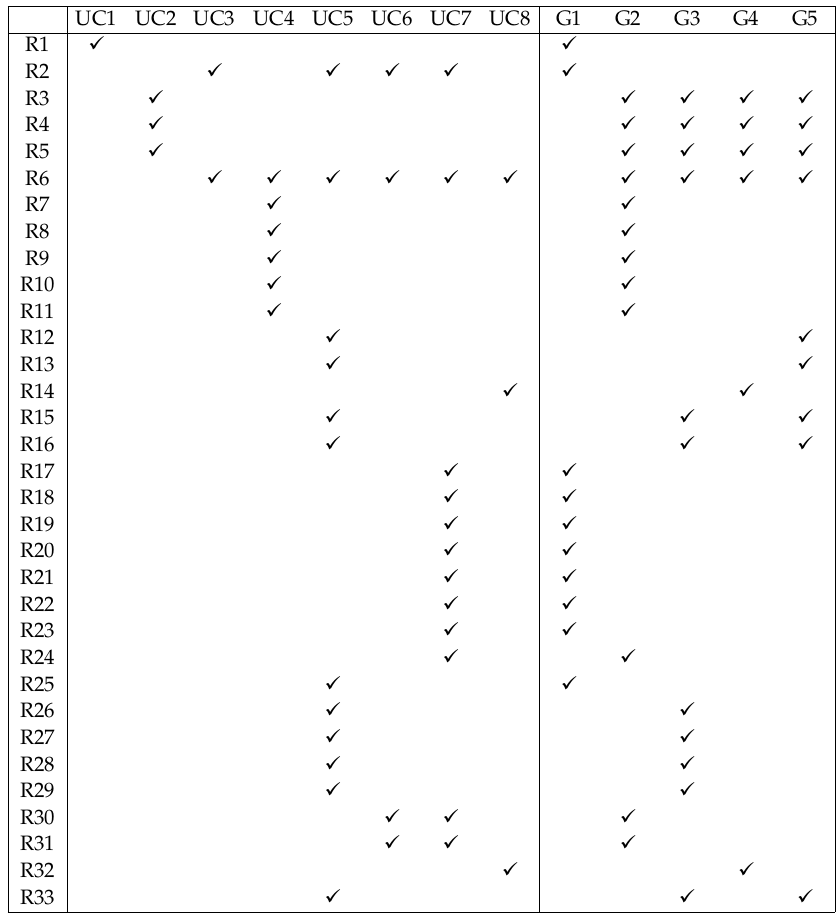
\includegraphics[scale=0.46]{trac_matrix-1.png} 
    \end{figure}
\newpage
\subsection{Performance Requirements}
Since the system does not need immediate responsiveness, the latency between components can also be in the order of seconds (e.g. 1 to 20 sec).\\
The amount of data produced by IoT sensors is significantly high, the system is expected to be able to process and classify all the data, thus having high storage capacities.\\
\textcolor{red}{To meet these requirements, the system is expected to be distributed in nature and have a Cloud infrastructure to rely on. \%forse non va inserito qua\%}
\subsection{Software System Attributes}
\subsubsection{Availability}
The target is to achieve an improved level of resilience with semi-automated recovery and to be taken offline for maintenance in agreed windows.
System relies on people that use it during the working hours, moreover, it is not needed to provide very high availability because the system is not strictly related with emergency situations.
According to these assumptions, the system should provide an Availability of 99.5\%.
\begin{center}
    \begin{tabular}{|c c c|} 
    \hline
    Availability \% & Downtime per year & Downtime per month\\ 
    \hline
    99.5\%  & 1.83 days & 3.6 hours\\ 
    \hline
    \end{tabular}
\end{center}
\subsubsection{Reliability}
The operations performed must be executed as intended as frequently as possible, in fact the probability that the data displayed is correct must be 
very high, so as not to compromise the evaluations performed by the actors in the system. To meet these requirements, the reliability of the system must 
not be less than 99.97\%.
\begin{center}
    \begin{tabular}{|c c c|} 
    \hline
    Reliability \% & Downtime per year & Downtime per month\\ 
    \hline
    99.97\%  & 2.63 hours & 13.14 minutes\\ 
    \hline
    \end{tabular}
\end{center}
\subsubsection{Security}
The data entered into the platform needs to be protected as it contains confidential information about telengana farmers. A secure communication channel and encryption of messages will be necessary.\\
Operations will always need to be authorized with an authentication mechanism, specifically the PM login mechanism must be 2FA (two-factor authentication).
\subsubsection{Maintainability}
The infrastructure needs thorough documentation of the code base to ensure that the underlying logic can be quickly understood by maintenance personnel.\\
Through the use of design patterns and best practices in the implementation, it will be easier to ensure future additions.
\subsubsection{Portability}
The client application, including the front-end and user interface, must be supported by Windows and Mac operating systems. \\
A mobile version of the client application is not planned.
\subsection{Design Constraints}
\subsubsection{Standards compliance}
In order to effectively store data into the DBMS and to easily retrieve significant information, the reports created by farmers will have to follow a standard model.
Particular attention is required when inserting the types of goods and auxiliary products in the report: these will have to be the same across different reports in order
to facilitate querying and data aggregation. In order to do this, the report form will guide farmers to insert correct data and avoid misalignments with the information stored 
in the DBMS: the ultimate goal is to prevent errors such as typos when compiling the report form and to avoid the insertion of data which is incoherent with the other reports. 
\end{document}
